\documentclass{beamer}

\mode<presentation> {


\usetheme{Szeged}

\usecolortheme{dolphin}


\setbeamertemplate{footline} % To remove the footer line in all slides uncomment this line
%\setbeamertemplate{footline}[page number] % To replace the footer line in all slides with a simple slide count uncomment this line

\setbeamertemplate{navigation symbols}{} % To remove the navigation symbols from the bottom of all slides uncomment this line
}

\usepackage[spanish, es-tabla, es-nodecimaldot]{babel}
%\usepackage[utf8]{inputenc}
\usepackage{mathrsfs}
\usepackage{amssymb, amsmath, amsthm}

% \usepackage{hyperref}
\usepackage{url}
\usepackage{textcomp}
\usepackage{gensymb}
%\usepackage[dvipsnames]{xcolor}

\usepackage{parskip}
\usepackage{fancyhdr}
\usepackage{multicol}
\usepackage{setspace}
\usepackage{geometry}

\usepackage{float}
\usepackage{array}
\usepackage{graphicx}
\graphicspath{{./images/}{../Documento/images/}}
\usepackage{wrapfig}
\usepackage{caption}
\usepackage{subcaption}

\usepackage{pstricks}
\newrgbcolor{darkgreen}{0 .5 0}
\newrgbcolor{blues}{0 0 .5}
\newrgbcolor{morado}{.3984 .1992 .9961}
\newrgbcolor{cafe}{.5391 .3594 .1797}
\newrgbcolor{cafeoscuro}{.4 .26 .13}
\newrgbcolor{darksienna}{0.24, 0.08, 0.08}
\newrgbcolor{apricot}{0.984, 0.808, 0.694}


\usepackage{booktabs} % Allows the use of \toprule, \midrule and \bottomrule in tables

%========================================================================================
%   TITLE PAGE
%========================================================================================

\title[Simulaciones de materia oscura]{Subestructura en simulaciones de materia oscura} % The short title appears at the bottom of every slide, the full title is only on the title page

\author{L.F. Martín Alejandro Paredes Sosa} % Your name
\institute[Universidad de Sonora MCF ] % Your institution as it will appear on the bottom of every slide, may be shorthand to save space
{
Universidad de Sonora\\ % Your institution for the title page
\medskip
% \textbf{Director}: Dr. Carlos Calcáneo Roldan \\
% \medskip
\tiny{Maestría en Ciencias (Física)}\\
%\textit{\tiny{mapsjr16@gmail.com}} % Your email address
\medskip
\tiny{Hermosillo, Sonora a Agosto, 2023 }
}
\date{} % Date, can be changed to a custom date

\usepackage{tikz}
\titlegraphic{
	\begin{tikzpicture}[overlay,remember picture]
		\node[left=0.5cm] at (current page.335){
	    
\includegraphics[width=2cm]{USON.png}   % LOGOTIPO
	};
\end{tikzpicture}


}
%========================================================================================%========================================================================================%========================================================================================

\begin{document}
{\setbeamertemplate{headline}{}
\begin{frame}
\titlepage % Print the title page as the first slide
%\vspace*{-2.0cm}
%%\includegraphics[scale= 1]{IA_UNAM.png}
%\hspace*{8.5cm}
%
\includegraphics[width= 0.2\linewidth]{USON.png}

\end{frame}

%========================================================================================
\begin{frame}
    \frametitle{Contenido}
    
    \begin{columns}[t]
        
        \begin{column}{.5\textwidth}
            \tableofcontents[sections={1-2}]
        \end{column}

        \begin{column}{.5\textwidth}
            \tableofcontents[sections={3-5}]

        \end{column}

    \end{columns}

\end{frame}
%\begin{frame}
%
%\vspace*{-0.25cm}
%	\frametitle{Contenido} % Table of contents slide, comment this block out to remove it
%	\tableofcontents % Throughout your presentation, if you choose to use \section{} and \subsection{} commands, these will automatically be printed on this slide as an overview of your presentation
%
%\end{frame}
}
\addtocounter{framenumber}{-1} %Restart frame counter

%========================================================================================
%   PRESENTATION SLIDES
%========================================================================================

\section{Introducción}
	\begin{frame}
		\frametitle{Introducción}
		
		En este trabajo resumimos los resultados de usar GADGET-4, el cual esta disponible para hacer simulaciones cosmológicas. Mi trabajo principal consistió en aprender a ajustar los modelos necesarios y correr distintos escenarios Cosmológicos para corroborar que las simulaciones pueden servir para discriminar el Universo en el que vivimos de una vasta posibilidad de modelos.
		\end{frame}


%========================================================================================
%========================================================================================
%========================================================================================
\section{Modelo Cosmológico}
	\begin{frame}
		\frametitle{Modelo Cosmológico}
		Existe una gran cantidad de evidencia de que el Universo tiene una componente no luminosa conocida como ``materia oscura'' y este no es la materia bariónica habitual (protones, neutrones, electrones, etc), sino alguna partícula cuyas propiedades son desconocidas.

Se han probado muchas escalas en la búsqueda de evidencia de materia oscura: desde la escala cosmológica hasta la escala local de galaxias. En el segundo de estos métodos es el mas favorable debido a que es relativamente mas sencillo extraer información dinámica de los sistemas cercanos. Experimentos en la escala cosmológica como el WMAP, la Misión Planck hacen posibles medidas detalladas de muchos parámetros cosmológicos.

	\end{frame}
	%========================================================================================

\subsection{Materia y Energía en el Universo}
	\begin{frame}
		La cantidad y composición de materia y energía en el Universo es de fundamental en la cosmología. Podemos descomponer la densidad de materia/energía en tres componentes: la aportada por la radiación ($\Omega_{rad}$), la componente de materia ($\Omega_{0}$) y una contribución suave ($\Omega_{\lambda}$).		
		\begin{equation}
			\Omega \equiv \frac{\rho_{tot}}{\rho_o} = \Omega_{rad} + \Omega_0 + \Omega_{\Lambda}
		\end{equation}
Esta elección trata de reflejar los valores medidos actuales, donde la materia y la radiación son componentes evidentes. La contribución de la radiación a la densidad total de energía en el Universo es pequeña,podemos continuar tomando en cuenta solamente $\Omega_{M}$ y $\Omega_{\Lambda}$, donde las observaciones apuntan a que $\Omega=1\pm 0.1$, $\Omega_{0}\approx 0.3$ y $\Omega_{\Lambda}\approx 0.7$.
	\end{frame}
	
%========================================================================================

\subsection{Evidencia astrofísica de la Materia Oscura}
	\begin{frame}
		Las primeras evidencias de la materia oscura, fueron en las mediciones de las velocidades de estrellas cercanas, donde concluyó que había de un $30\%$ a $50\%$ mas de materia gravitante de la que es visible. También del estudio de dispersión de velocidades del cúmulo ricos de galaxias requieren de $10$ a $100$ mas masa para que se encuentren unidas. 
		
		Estos ejemplos nos ilustran como la dinámica de estrellas, galaxias y cúmulos sirven como una sonda para detectar el contenido de materia en el Universo.


	\end{frame}
%========================================================================================
\subsection{Características de la Materia Oscura}

	\begin{frame}
			La mayor parte de la materia del Universo es ``materia oscura'', la cual no interactúa con los campos electromagnéticos y solo la podemos detectarla por su interacción gravitacional y posiblemente por su interacciones de fuerza débil. Sus efectos sobre la materia ordinaria son espectaculares dado que los pozos de potencial gravitacional de materia oscura canalizan a los bariones formando los lugares de nacimiento de las galaxias visibles. El estudio de estos lugares nos permite estudiar el crecimiento de estructuras de materia oscura conocidas como ``halos''.

	\end{frame}

%========================================================================================

	\begin{frame}
		El estudio de los halos no es simple y aunque no existe un consenso en la definición de sus propiedades, pero lo definen como un objeto ligado gravitacionalmente. Algunas propiedades con la que caracterizan los halos son la masa, velocidad circular, dispersión de velocidades del halo, el radio que contiene la mitad de la masa y el radio  de la velocidad maxima. Sin embargo, cada una de estas cantidades puede referirse a distintos aspectos físicos de la colección de partículas a la que llamamos halos.
	\end{frame}

%========================================================================================
%====================== Simulaciones Cosmológicas =======================================
%========================================================================================
\section{Simulaciones cosmológicas}
	\begin{frame}
		\frametitle{Simulaciones Cosmológicas}
		Las simulaciones cosmológicas son una herramienta esencial para el estudio del Universo. Son el único experimento con el que contamos para reproducir su evolución. Estas permiten un estudio detallado de estructura y nos permite hacer conexiones entre un Universo simple con alto corrimiento al rojo, con un Universo complejo como en la actualidad.
		
		Gracias al desarrollo de códigos y el avance en el hardware de las maquinas modernas, han surgido grandes colaboraciones con la intención de realizar simulaciones cada vez mas grandes. Algunas de estas colaboraciones son la \textit{Millennium Simulation} y la \textit{Eagle Simulation}.
	\end{frame}
%========================================================================================
\subsection[La interacción dominante en las simulaciones]{La interacción Dominante}
	\begin{frame}
		La fuerza que se utiliza en las simulaciones es la gravedad descrita por Newton.
		\begin{equation}
		    F = G \frac{m_1 m_2}{r^2}
		    \label{eq:Gravedad-Newton}
		\end{equation}
		También se suele resolver trabajando el problema con el potencial
		\begin{equation}
		    \nabla \phi(\mathbf{r}) = \mathbf{F}
		    \label{eq:potencial-gravitacional}
		\end{equation}
	\end{frame}
	

%========================================================================================
\subsection[Una razón práctica para las simulaciones]{Razón de las Simulaciones}

	\begin{frame}
		Dado que en el Universo las colisiones son eventos raros, podemos modelar al Universo usando la  ecuación de Boltzmann sin colisiones (CBE)
	
		
		\begin{equation}
		    \frac{d f}{d t} \equiv \frac{\partial f}{\partial t} + \mathbf{v}\frac{\partial f}{\partial \mathbf{x}} + \frac{\partial \Phi}{\partial \mathbf{r}} \frac{\partial f}{\partial \mathbf{v}}
		    \label{eq:CBE}
		\end{equation}

		donde el potencial auto-consistente $\Phi$ es la solución a la ecuación de Poisson

		\begin{equation}
		    \nabla^2\Phi(\mathbf{r},t) = 4\pi G \int f(\mathbf{r},\mathbf{v},t)d\mathbf{v}
		    \label{eq:PoissonSol}
		\end{equation}
		\noindent y $f(\mathbf{r},\mathbf{v},t)$ es la densidad de partículas en el espacio fase.
	\end{frame}
	
	\begin{frame}
		Sin embargo, la dinámica se suele aproximar mediante códigos de N-cuerpos, en el cual supone una interacción entre las partículas dada por la interacción gravitacional clásica por pares de partículas a las que se les agrega un radio de suavizado.

		 La diferencia entre códigos suele estar en los métodos que usan para realizar los cálculos para el movimiento gravitacional, asi como la manera en la que buscan volverlos mas rápidos y eficientes.

	\end{frame}
%========================================================================================
\subsection{GADGET-4}
	\begin{frame}
		El código GADGET es uno de los mas utilizados en el estudio de formación de estructura y estudio de materia oscura. Una de las características que separa a GADGET de otros simuladores, es que es un código flexible multi-propósito que no restringe el tipo de simulaciones, sino que da prioridad a la flexibilidad sobre la optimización para casos específicos.
		
		En GADGET-4 se implementaron nuevos métodos numéricos y se introdujeron nuevas herramientas como el FOF y sus variaciones, un generador de condiciones iniciales, entre otras.

	\end{frame}
	
	
	\begin{frame}
		El potencial que se resuelve en GADGET-4 es 
		\begin{align}
    \Phi (\textbf{x}) = &- \sum_{j=1}^{N} \frac{m_j}{|\textbf{x}_j-\textbf{x}+\textbf{q}^*_j| + |\epsilon(\textbf{x}_j-\textbf{x}+\textbf{q}^*_j)|} \nonumber \\
    &+ \sum_{j=1}^{N} m_j \psi (\textbf{x}_j-\textbf{x}+\textbf{q}^*_j) \label{eq:Pot}
\end{align}
		donde la primera parte es el potencial gravitacional de newton con una corrección para considerar el radio de suavizado y el segundo termino en potencial se introduce como una corrección para el suavizado de imágenes distantes. Como GADGET es un simulador diseñado para abarcar una amplia gama de necesidades, se implementaron diversos algoritmos para la forma en la que se realizan los cálculos.
	\end{frame}
	
	\begin{frame}
		En GADGET-4 se han implementado una diversa cantidad de herramientas con las que podemos estudiar nuestras simulaciones y muchas de estas corren junto a la simulación, lo que permite tener mejores resultados. Algunas de las herramientas que se implementaron son buscadores de grupos, constructores de arboles de fusión, conos de luz, entre otros.
	\end{frame}
	
	\begin{frame}
		GADGET-4 tiene diversas implementación es de grupos y sub-halos. Se introdujeron versiones propias de FOF y SUBFIND, ademas se creo SUBFIND-HBT (Hierarchically Bound Tracing). FOF busca partículas cercanas, mientras que SUBFIND verifica que las estructuras encontradas estén ligadas gravitacionalmente y SUBFIND-HBT hace el mismo estudio pero en el espacio fase y considera las afiliaciones pasadas.
	
	\end{frame}


%========================================================================================
%========================================================================================
%========================================================================================
\section{Halos de Materia Oscura}
\setcounter{equation}{0}
	\begin{frame}
		\frametitle{Halos de Materia Oscura}
		Con la intención de conocer y diferenciar diferentes cosmologías, en nuestro estudio de los halos de materia oscura, optamos por realizar fue una variedad de simulaciones de materia oscura. Desde simulaciones con cosmologías de Universos planos ($\Omega=1$), asi como cosmologías de universos con densidades sub-criticas ($\Omega < 1$) y super-criticas ($\Omega > 1$). Las simulaciones que realizamos tienen $16,777,216$ partículas en una caja de $50$ Mpc y se empezaron con un corrimiento al rojo de $z = 63$ hasta un $z = 0$.
		
	\end{frame}
%========================================================================================
\subsection{Cosmología \texorpdfstring{$\Omega_\lambda = 0.691$ $\Omega_0 = 0.309$}{Omega lambda = 0.691, Omega 0 = 0.309} }
	\begin{frame}
		\frametitle{Universo $\Omega_\lambda=0.691$, $\Omega_0=0.309$}
		\begin{columns}[t]
           	\begin{column}{.5\textwidth}

				\begin{figure}
					\centering
					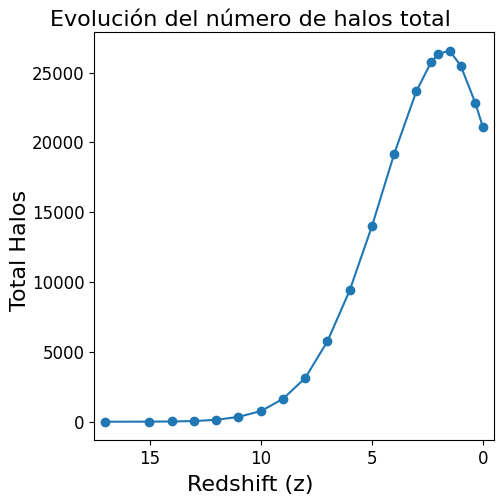
\includegraphics[scale=0.38]{RunCanonica/TotalHalos_RunCanonica.png}
					\caption{\footnotesize Se muestra el numero de halos según el redshift y podemos observar como evoluciona el Universo en una cosmología $\Omega_\lambda = 0.691 $ y $\Omega_0 = 0.309$.}
					\label{fig:TotalHalos_CanonRun}
				\end{figure}

	        \end{column}
			\vspace{0.5cm}
    	    \begin{column}{.5\textwidth}

    	    	Esta es la cosmología con la distribución de densidades mas aceptada de nuestro Universo. Las estructuras que se forman empiezan a aparecer en $z=17$, pero a partir de $z=10$ se ve un incremento significante en la cantidad de halos hasta alcanzar un máximo 26,584 halos en $z = 1.5$ y finalizando en $z=0$ con 21,097 halos.

        	\end{column}
	    \end{columns}

	\end{frame}
%========================================================================================

	\begin{frame}
			\small Observamos que la masa media incrementa desde $10^{10.41}M_\odot$ con una desviación de $10^{0.11}M_\odot$ en $z=15$ hasta $10^{10.75}M_\odot$ con una desviación de $10^{0.49}M_\odot$ en $z=0$.
		\begin{columns}[t]
			\begin{column}{.5\textwidth}
				\begin{figure}
					\centering
					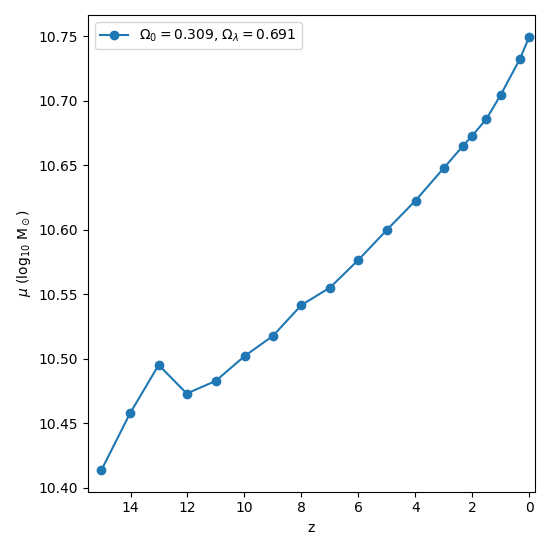
\includegraphics[scale=0.3]{RunCanonica/MassMean_RunCanonica.png}
					\caption{\footnotesize La evolución de la masa media de los halos de materia oscura en el Universo desde un z=17 hasta z=0.}
					\label{fig:Canon-MassMean}
				\end{figure}
			\end{column}
			
			\begin{column}{.5\textwidth}
				\begin{figure}
					\centering
					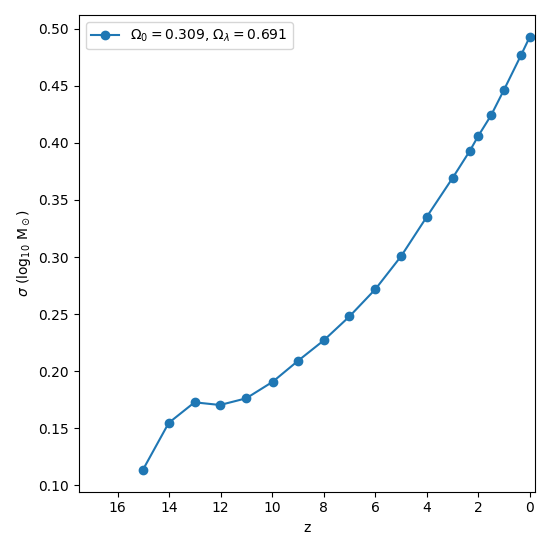
\includegraphics[scale=0.3]{RunCanonica/MassStd_RunCanonica.png}
					\caption{\footnotesize La evolución de la desviación estándar de la masa de los halos de materia oscura en el Universo desde un z=17 hasta z=0.}
					\label{fig:Canon-MassStd}
				\end{figure}
			\end{column}
		\end{columns}

	\end{frame}	

%========================================================================================
	\begin{frame}
		\small Vemos el crecimiento del radio medio desde $10^{0.44}$kpc con una desviación de $10^{0.06}$kpc en $z=15$ hasta un radio de $10^{1.47}$kpc con una desviación de $10^{0.19}$kpc en $z=0$.
		
		\begin{columns}[t]
			\begin{column}{.5\textwidth}
				\begin{figure}
					\centering
					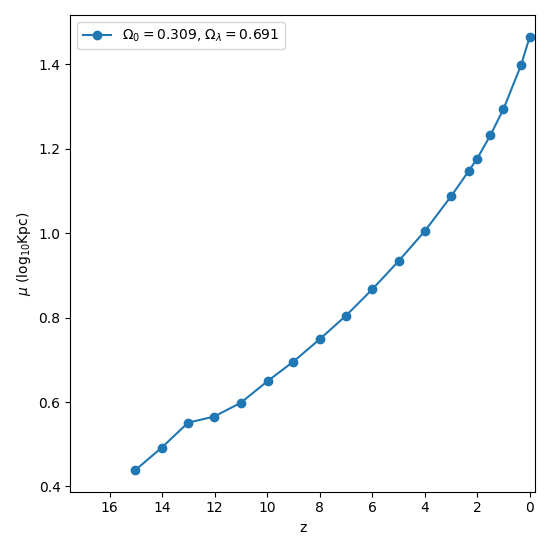
\includegraphics[scale=0.3]{RunCanonica/HalfMassRad_Mean_RunCanonica.png}
					\caption{\footnotesize La evolución del radio que contiene la mitad de la masa de los halos de materia oscura desde un z=17 hasta z=0.}
					\label{fig:Canon-HalfMassRadMean}
				\end{figure}
			\end{column}

			\begin{column}{.5\textwidth}
				\begin{figure}
					\centering
					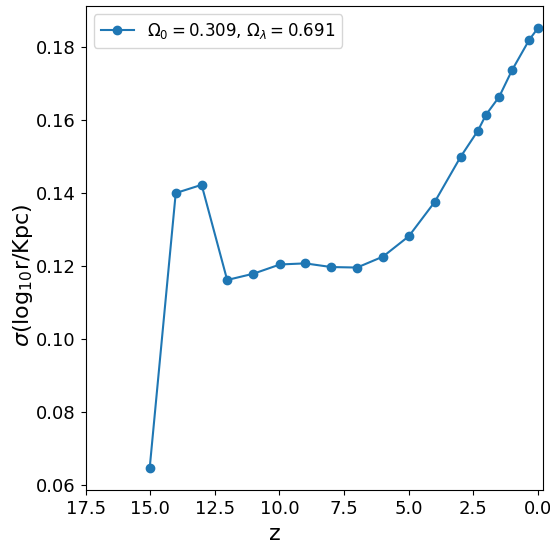
\includegraphics[scale=0.3]{RunCanonica/HalfMassRad_Std_RunCanonica.png}
					\caption{\footnotesize La evolución de la desviación estándar del radio que contiene la mitad de la masa de los halos de materia oscura desde un z=17 hasta z=0.}
					\label{fig:Canon-HalfMassRadStd}
				\end{figure}
			\end{column}
		\end{columns}

	\end{frame}	

%========================================================================================
	\begin{frame}
		\small Vemos que el radio tiene una media que va desde los $2.45$kpc con una desviación de $0.88$kpc en $z=15$ hasta $27.60$kpc con una desviación de $15.69$kpc en $z=0$.
		
		\begin{columns}[t]
			\begin{column}{.5\textwidth}
				\begin{figure}
					\centering
					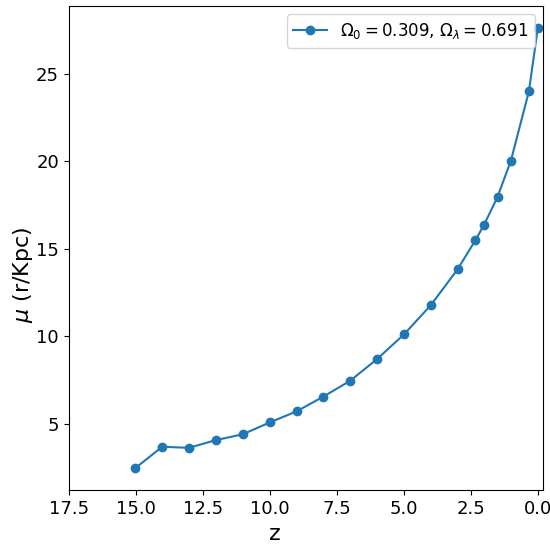
\includegraphics[scale=0.3]{RunCanonica/VMaxRad_Mean_RunCanonica.png}
					\caption{\footnotesize La evolución del radio donde se alcanza la velocidad máxima radial de los halos de materia oscura desde un z=17 hasta z=0.}
					\label{fig:Canon-VMAxRadMean}
				\end{figure}
			\end{column}

			\begin{column}{.5\textwidth}
				\begin{figure}
					\centering
					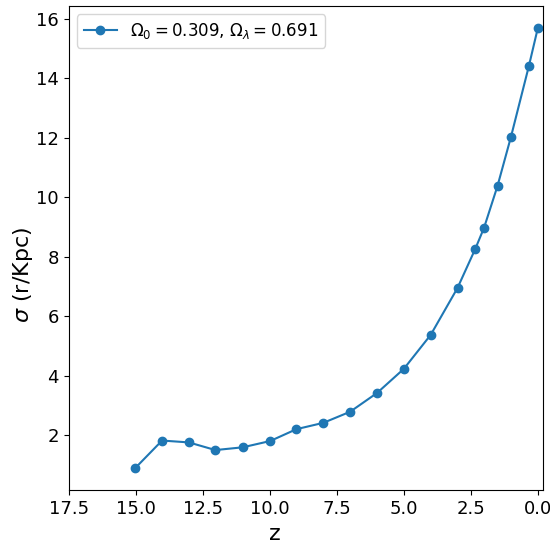
\includegraphics[scale=0.3]{RunCanonica/VMaxRad_Std_RunCanonica.png}
					\caption{\footnotesize La evolución de la desviación estándar del radio de la velocidad máxima radial de los halos de materia oscura desde un z=17 hasta z=0.}
					\label{fig:Canon-VMaxRadStd}
				\end{figure}
			\end{column}
		\end{columns}

	\end{frame}	

%========================================================================================

	\begin{frame}
		\small Lo que podemos es que la velocidad media disminuye rápidamente desde $150.13$km/s con una desviación de $26.76$km/s en $z=15$ hasta que alcanza $74.77$km/s con una desviación de $33.90$km/s en $z=0$.
		
		\begin{columns}[t]
			\begin{column}{.5\textwidth}
				\begin{figure}
					\centering
					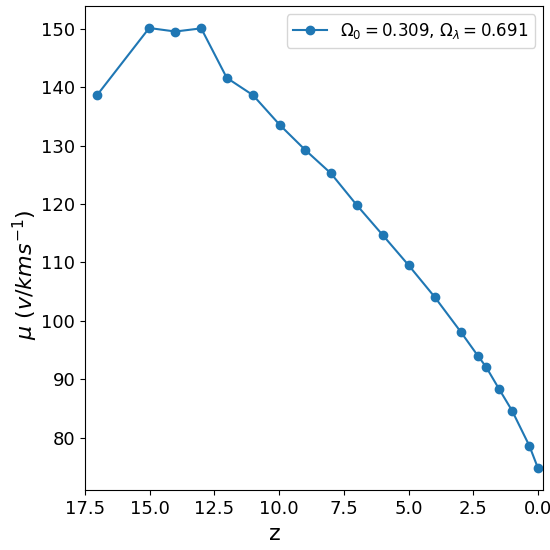
\includegraphics[scale=0.3]{RunCanonica/VelMax_Mean_RunCanonica.png}
					\caption{\footnotesize La evolución de la velocidad máxima circular media de los halos de materia oscura desde un z=17 hasta z=0.}
					\label{fig:Canon-VelMaxMean}
				\end{figure}
			\end{column}

			\begin{column}{.5\textwidth}
				\begin{figure}
					\centering
					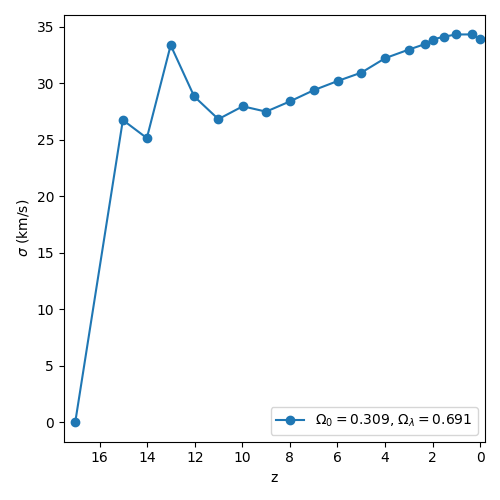
\includegraphics[scale=0.3]{RunCanonica/VelMax_Std_RunCanonica.png}
					\caption{\footnotesize La evolución de la desviación estándar de la velocidad máxima circular de los halos de materia oscura desde un z=17 hasta z=0.}
					\label{fig:Canon-VelMaxStd}
				\end{figure}
			\end{column}
		\end{columns}

	\end{frame}	

%========================================================================================

	\begin{frame}
		\small Observamos que la dispersión de velocidades media disminuye desde los $85.25$km/s con una desviación de $13.09$km/s en $z=15$ a $37.08$km/s con una desviación de $18.69$km/s en $z=0$.
		
		\begin{columns}[t]
			\begin{column}{.5\textwidth}
				\begin{figure}
					\centering
					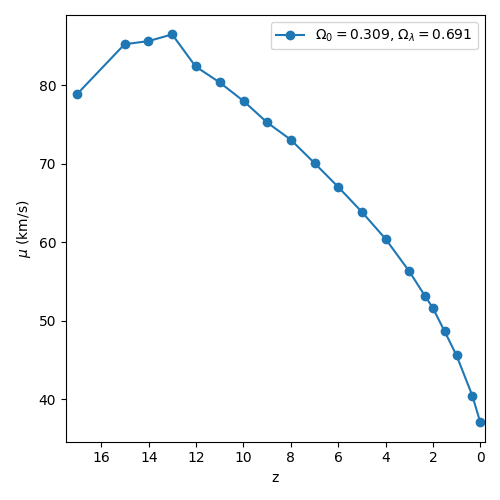
\includegraphics[scale=0.3]{RunCanonica/VelDisp_Mean_RunCanonica.png}
					\caption{\footnotesize La evolución de la dispersión de velocidades de los halos de materia oscura desde un z=17 hasta z=0.}
					\label{fig:Canon-VelDispMean}
				\end{figure}
			\end{column}

			\begin{column}{.5\textwidth}
				\begin{figure}
					\centering
					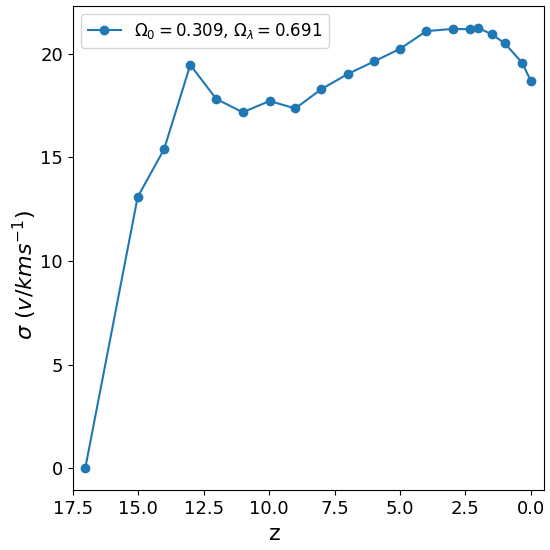
\includegraphics[scale=0.3]{RunCanonica/VelDisp_Std_RunCanonica.png}
					\caption{\footnotesize La evolución de la desviación estándar del radio de la dispersión de velocidades de los halos de materia oscura desde un z=17 hasta z=0.}
					\label{fig:Canon-VelDispStd}
				\end{figure}
			\end{column}
		\end{columns}

	\end{frame}	

%========================================================================================

\begin{frame}{Mapa de Densidad}

	\small Se muestra el mapa de densidad durante su evolución.  Los redshifts que se muestran son $z=63$, $z=10$ y $z=0$. Se observa evoluciona a lo que llaman \textit{Cosmic Web}.

	\begin{columns}[t]

		\begin{column}{0.33\textwidth}
			
			\begin{figure}
				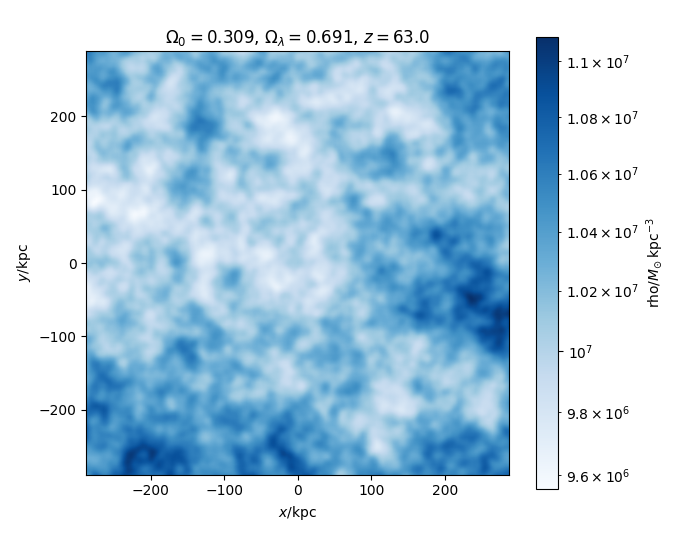
\includegraphics[scale=0.2]{RunCanonica/RunCanonZ63Rho.png}
				\caption{\footnotesize Mapa de densidad en $z=63$}
			\end{figure}

		\end{column}

		\begin{column}{0.33\textwidth}
			
			\begin{figure}
				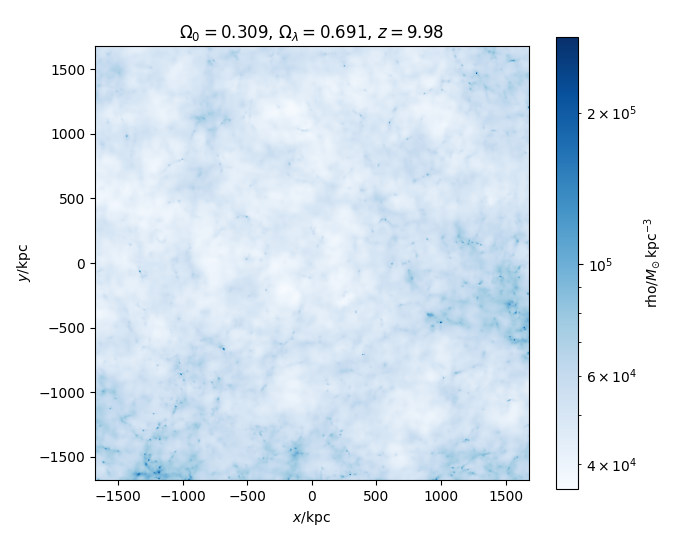
\includegraphics[scale=0.2]{RunCanonica/RunCanonZ10Rho.png}
				\caption{\footnotesize Mapa de densidad en $z=10$}
			\end{figure}

		\end{column}	

		\begin{column}{0.33\textwidth}
			
			\begin{figure}
				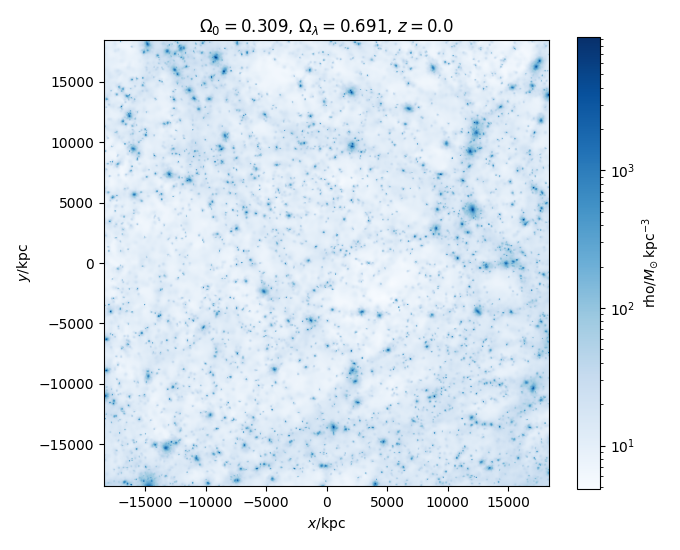
\includegraphics[scale=0.2]{RunCanonica/RunCanonZ0Rho.png}
				\caption{\footnotesize Mapa de densidad en $z=0$}
			\end{figure}

		\end{column}		
		
	\end{columns}
\end{frame}

%========================================================================================



%========================================================================================
\subsection{Comparando Cosmologías}
	\begin{frame}
		\frametitle{Comparando Cosmologías}
		\begin{columns}[t]
           	\begin{column}{.5\textwidth}

				\begin{figure}
					\centering
					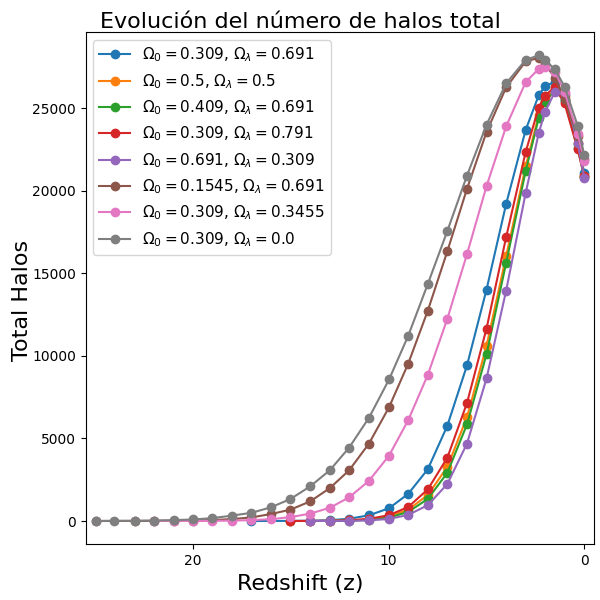
\includegraphics[scale=0.31]{Conc/TotalHalos_Conc.png}
					\caption{\footnotesize Se muestra el numero de halos según el redshift y podemos observar como evolucionan diferentes cosmologías }
					\label{fig:TotalHalos_Conc}
				\end{figure}

	        \end{column}
%			\vspace{0.5cm}
    	    \begin{column}{.5\textwidth}

    	    	Lo que podemos observar, es que las simulaciones sub-críticas se forma estructura mucho antes que el resto, alrededor de $z=25$ y forman una mayor cantidad de halos, aproximadamente $28,000$ halos.
    	    	
    	    	En el resto de las simulaciones, estas empieza a formar halos en $z=15$ donde alcanzan un máximo de halos entre $25,900$ y $26,300$.

        	\end{column}
	    \end{columns}

	\end{frame}
%========================================================================================

	\begin{frame}
			\only<1>{\small Vemos que la masa media en $\Omega_0=0.691$ $\Omega_\lambda=0.309$ tiene las estructuras mas masivas y $\Omega_0=0.1545$ $\Omega_\lambda=0.691$ las menos. }
			\only<2>{\small En las cosmologías sub-críticas, se ve que la desviación es mayor que en el resto, las cuales tienen un comportamiento similar.}
		\begin{columns}[t]
			\begin{column}{.5\textwidth}
				\begin{figure}
					\centering
					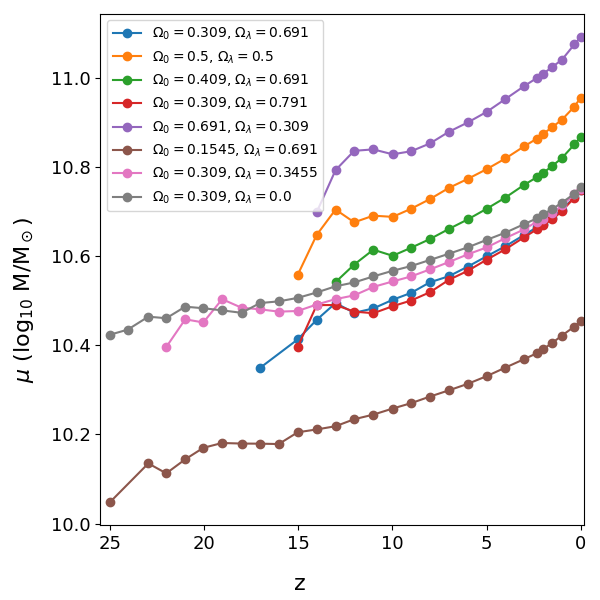
\includegraphics[scale=0.27]{Conc/MassMean_Conc.png}
					\caption{\footnotesize La evolución de la masa media de los halos de materia oscura en diferentes cosmologías.}
					\label{fig:Conc-MassMean}
				\end{figure}
			\end{column}
			
			\begin{column}{.5\textwidth}
				\begin{figure}
					\centering
					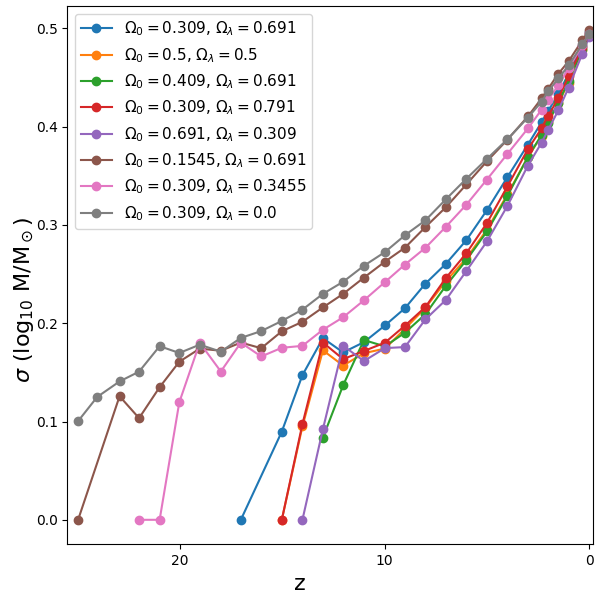
\includegraphics[scale=0.27]{Conc/MassStd_Conc.png}
					\caption{\footnotesize La evolución de la desviación estándar de la masa de los halos de materia oscura en diferentes cosmologías.}
					\label{fig:Conc-MassStd}
				\end{figure}
			\end{column}
		\end{columns}

	\end{frame}	

%========================================================================================
	\begin{frame}
		\only<1> {\small Vemos que la media del radio der las diferentes cosmologías tienen un crecimiento similar, donde las cosmologías con un incremento $\Omega_0$ son las de mayor radio y las sub-críticas son las de menor.}
		\only<2>{\small Mientras la desviación estándar del radio, muestra que las cosmologías sub-críticas tienen mayor variación en las cosmologías sub-críticas.}
		
		\begin{columns}[t]
			\begin{column}{.5\textwidth}
				\begin{figure}
					\centering
					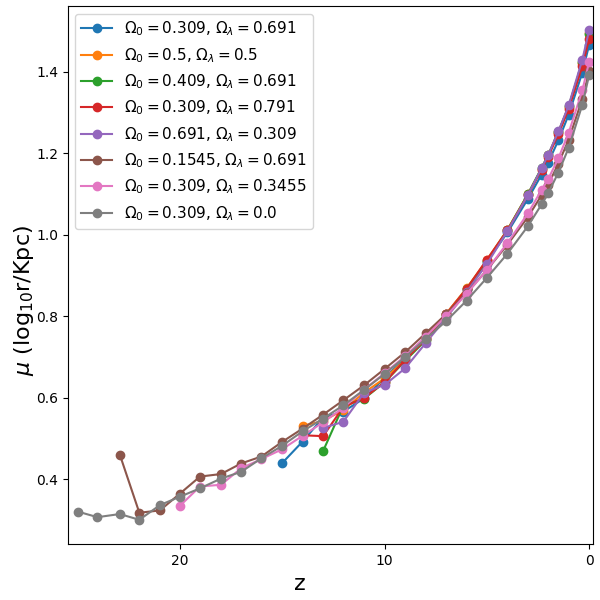
\includegraphics[scale=0.27]{Conc/HalfMassRad_Mean_Conc.png}
					\caption{\footnotesize La evolución del radio que contiene la mitad de la masa de los halos de materia oscura en diferentes cosmologías.}
					\label{fig:Conc-HalfMassRadMean}
				\end{figure}
			\end{column}

			\begin{column}{.5\textwidth}
				\begin{figure}
					\centering
					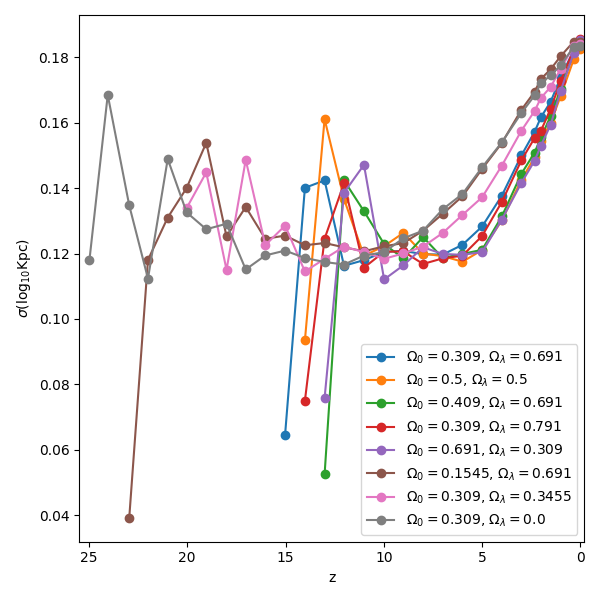
\includegraphics[scale=0.27]{Conc/HalfMassRad_Std_Conc.png}
					\caption{\footnotesize La evolución de la desviación estándar del radio que contiene la mitad de la masa de los halos de materia oscura en diferentes cosmologías.}
					\label{fig:Conc-HalfMassRadStd}
				\end{figure}
			\end{column}
		\end{columns}

	\end{frame}	

%========================================================================================
	
	\begin{frame}
		\only<1> {\small Se observa que con el incremento de $\Omega_0$ las estructuras alcanzan un mayor radio medio, mientras en los Universos sub-críticos los radios son lo mas pequeños. }
		\only<2> {\small Un caso especial que se ve fue que la cosmología con $\Omega_\lambda=0.791$ tiene un crecimiento similar a cuando $\Omega_0$ crece.}
		\only<2> {\small En cuanto a su desviación, vemos el mismo comportamiento que la media al incrementar $\Omega_0$ }
		
		\begin{columns}[t]
			\begin{column}{.5\textwidth}
				\begin{figure}
					\centering
					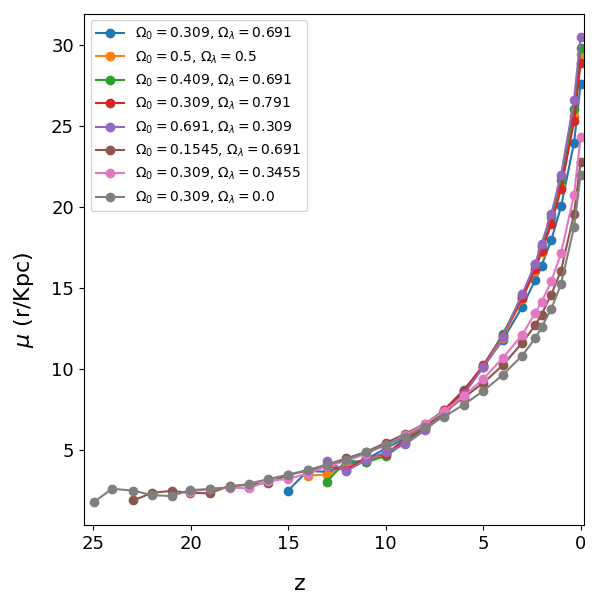
\includegraphics[scale=0.27]{Conc/VMaxRad_Mean_Conc.png}
					\caption{\footnotesize La evolución del radio donde se alcanza la velocidad máxima radial de los halos de materia oscura en diferentes cosmologías.}
					\label{fig:Conc-VMAxRadMean}
				\end{figure}
			\end{column}

			\begin{column}{.5\textwidth}
				\begin{figure}
					\centering
					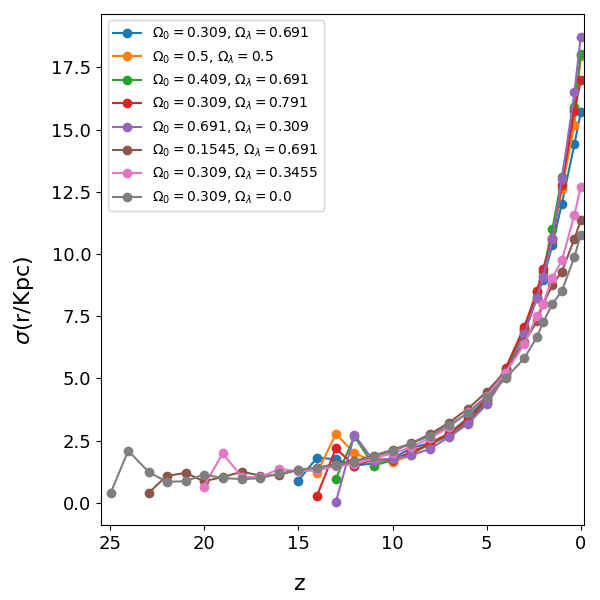
\includegraphics[scale=0.27]{Conc/VMaxRad_Std_Conc.png}
					\caption{\footnotesize La evolución de la desviación estándar del radio de la velocidad máxima radial de los halos de materia oscura en diferentes cosmologías.}
					\label{fig:Conc-VMaxRadStd}
				\end{figure}
			\end{column}
		\end{columns}

	\end{frame}	

%========================================================================================

	\begin{frame}
		\only<1> {\small Podemos notar que entre mas grande sea el $\Omega_0$, los halos que se forman alcanzan una mayor velocidad maxima media.}
				
		\begin{columns}[t]
			\begin{column}{.5\textwidth}
				\begin{figure}
					\centering
					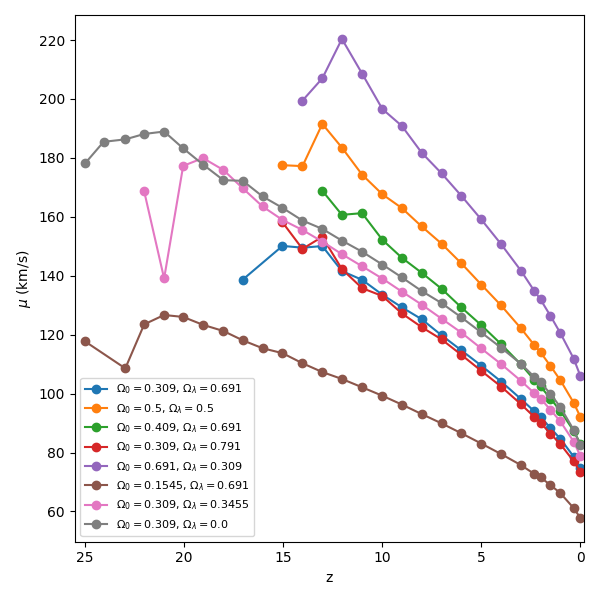
\includegraphics[scale=0.27]{Conc/VelMax_Mean_Conc.png}
					\caption{\footnotesize La evolución de la velocidad máxima circular media de los halos de materia oscura en diferentes cosmologías.}
					\label{fig:Conc-VelMaxMean}
				\end{figure}
			\end{column}

			\begin{column}{.5\textwidth}
				\begin{figure}
					\centering
					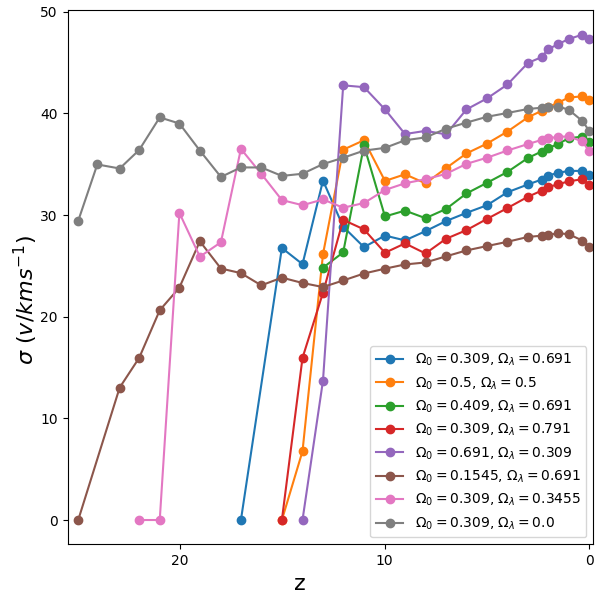
\includegraphics[scale=0.27]{Conc/VelMax_Std_Conc.png}
					\caption{\footnotesize La evolución de la desviación estándar de la velocidad máxima circular de los halos de materia oscura en diferentes cosmologías.}
					\label{fig:Conc-VelMaxStd}
				\end{figure}
			\end{column}
		\end{columns}

	\end{frame}	

%========================================================================================

	\begin{frame}
		\small Podemos apreciar que la dispersión de velocidades media se ve afectado con el aumento de $\Omega_0$ de la misma manera que la velocidad maxima.
		
		\begin{columns}[t]
			\begin{column}{.5\textwidth}
				\begin{figure}
					\centering
					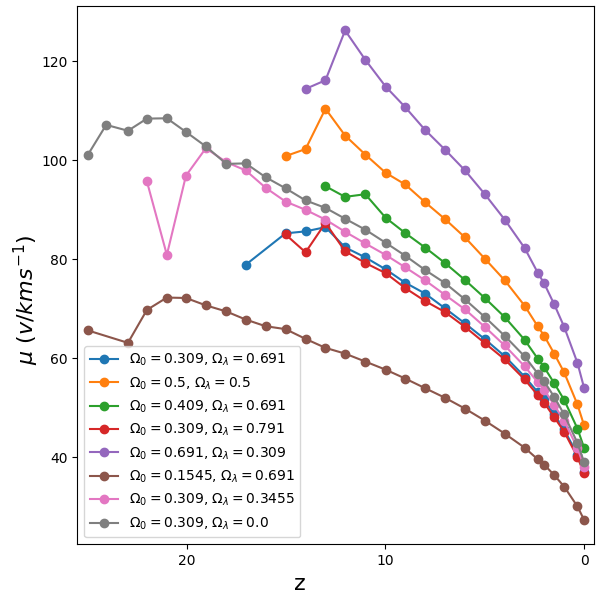
\includegraphics[scale=0.27]{Conc/VelDisp_Mean_Conc.png}
					\caption{\footnotesize La evolución de la dispersión de velocidades de los halos de materia oscura en diferentes cosmologías.}
					\label{fig:Conc-VelDispMean}
				\end{figure}
			\end{column}

			\begin{column}{.5\textwidth}
				\begin{figure}
					\centering
					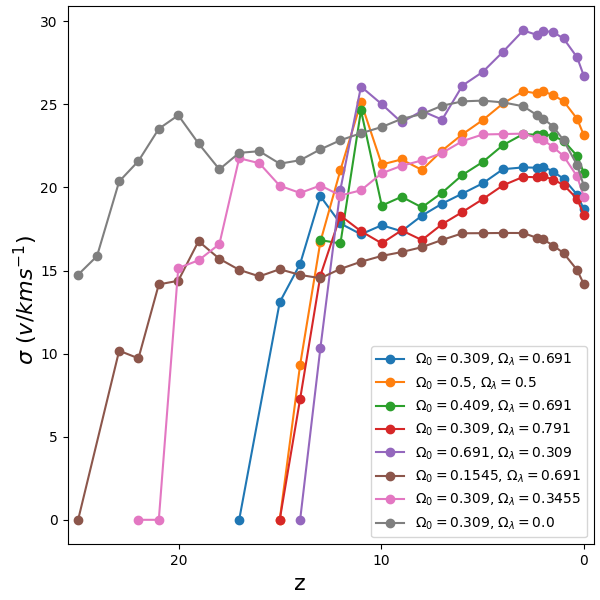
\includegraphics[scale=0.27]{Conc/VelDisp_Std_Conc.png}
					\caption{\footnotesize La evolución de la desviación estándar del radio de la dispersión de velocidades de los halos de materia oscura en diferentes cosmologías.}
					\label{fig:Conc-VelDispStd}
				\end{figure}
			\end{column}
		\end{columns}

	\end{frame}	

%========================================================================================

\begin{frame}

	\begin{figure}[H]
    	\centering

	    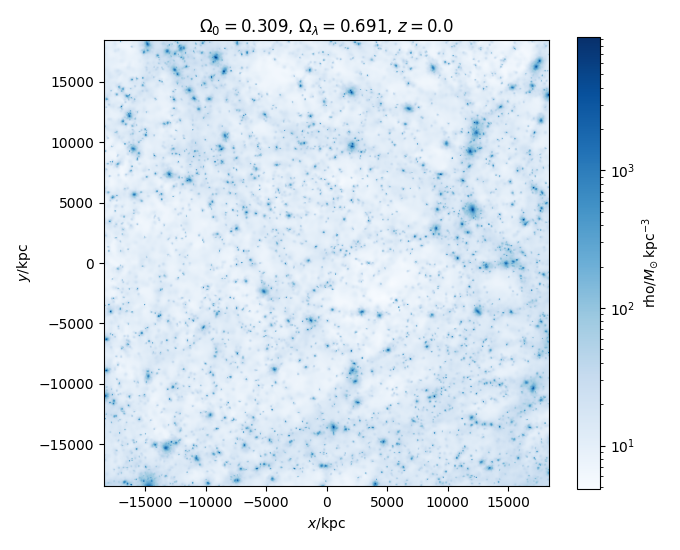
\includegraphics[width = 0.25\linewidth]{RunCanonica/RunCanonZ0Rho.png}   %Canon
	    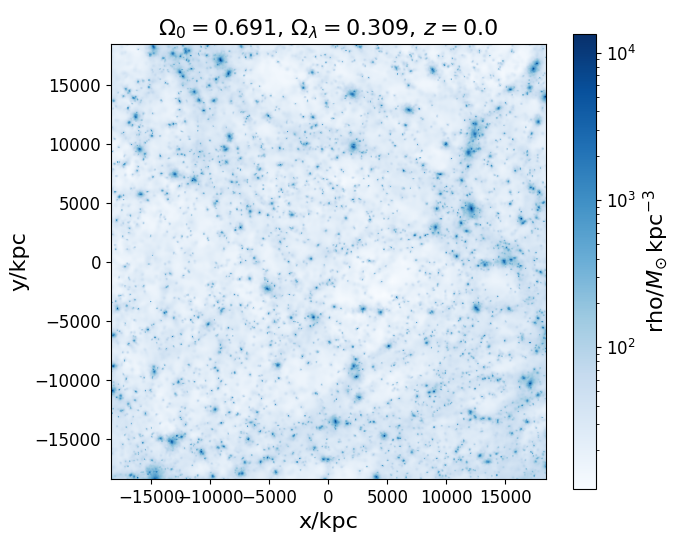
\includegraphics[width = 0.25\linewidth]{RunInvertida/RunInvertidaZ0.png}   %Invertida
	    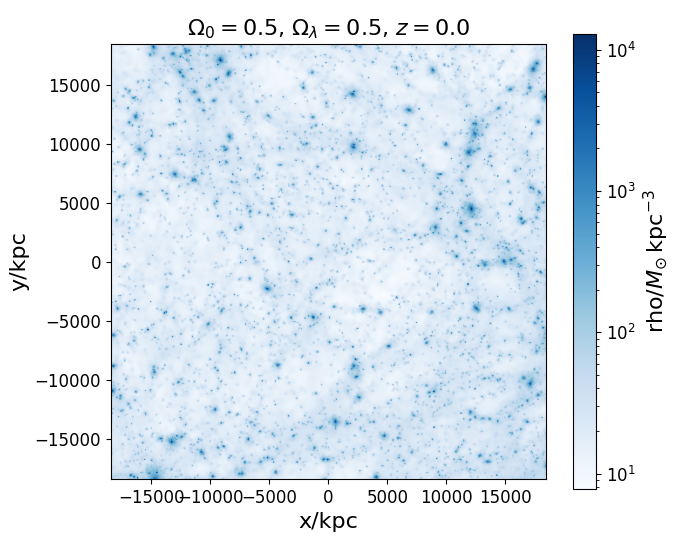
\includegraphics[width = 0.25\linewidth]{RunHalfCosmo/RunHalfCosmoZ0.png}   %HalfCosmo
	     \\
	    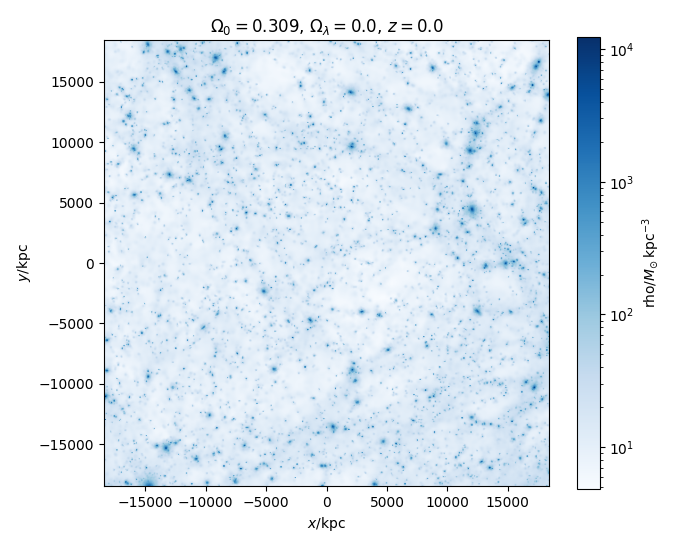
\includegraphics[width = 0.25\linewidth]{RunNoDE/RunNoDEZ0.png}   %NoDE
	    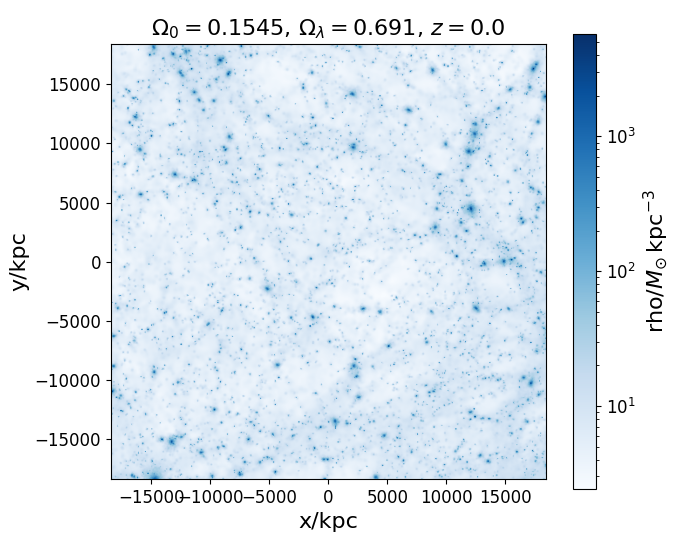
\includegraphics[width = 0.25\linewidth]{RunLow0/RunLow0Z0.png}   %Low0
	    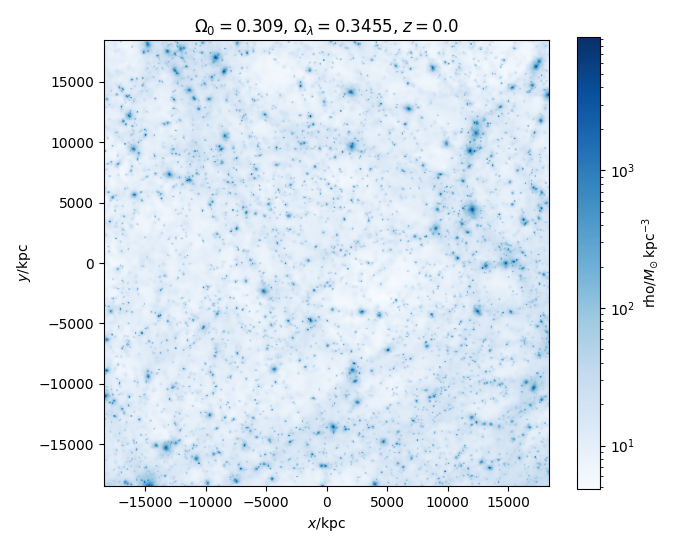
\includegraphics[width = 0.25\linewidth]{RunLowLam/RunLowLamZ0.png}    %LowLam
	    \\
	    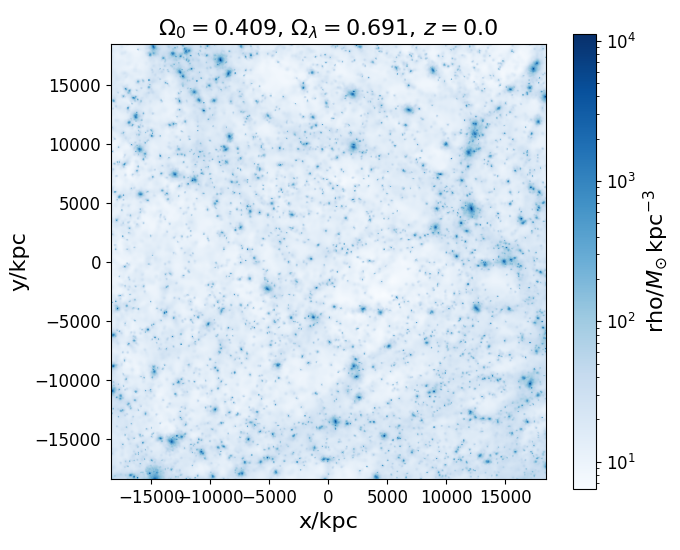
\includegraphics[width = 0.25\linewidth]{RunHigh0/RunHigh0Z0.png}    %High0
	    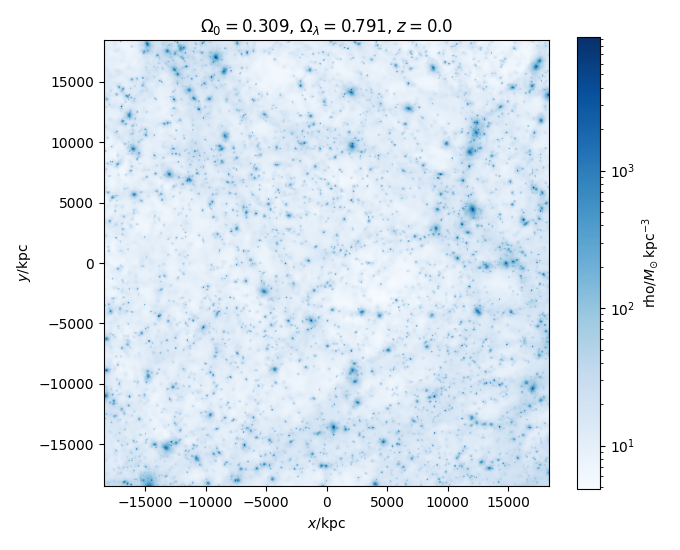
\includegraphics[width = 0.25\linewidth]{RunHighLam/RunHighLamZ0.png}  %HighLam
	    \caption{\footnotesize Mapa de densidad de las diferentes simulaciones. Cosmologías criticas en la parte superior, luego están las sub-críticas y las inferiores son super-críticas. }
    	\label{fig:DensityMap}
\end{figure}

\end{frame}




%=================================================================================
%=========================== Conclusion ==========================================
%=================================================================================
%y que la cosmología $\Omega_0 = 0.691$, $\Omega_\lambda = 0.309$ tiene grandes estructuras de gran masa que alcanzan grandes velocidades.
\section{Conclusión}
	\begin{frame}
		\frametitle{Conclusión}
Podemos ver que las velocidades se ven alteradas por los cambios en $\Omega_0$, mientra que el tamaño y la masa se ven afectadas por los cambios en $\Omega_0$ y en el tipo de cosmología, ya sea un Universos cerrado, abierto o plano. Pudimos observar que las cosmologías sub-críticas forman estructuras mas pequeñas y menos densas que el resto de las cosmologías.

Con este trabajo podemos inferir como es el comportamiento en la evolución de un Universo según sea sus densidades de materia y energía. Esto nos ayuda a poder inferir que tipo de Universo es en el que vivimos ya que podemos usar las observaciones y compararlas con resultados como estos para inferir las densidades del Universo.

	\end{frame}

\end{document}



%========================================================================================
